\documentclass[letter,11pt]{article}

\usepackage[spanish,es-nodecimaldot]{babel}
\usepackage[utf8]{inputenc}

\usepackage{lmodern}
\usepackage[T1]{fontenc}
\usepackage{textcomp}

\usepackage{framed}
\usepackage[svgnames]{xcolor}
\colorlet{shadecolor}{Gainsboro!50}

\usepackage[labelfont=bf]{caption}
\usepackage{graphicx}
\usepackage{pstricks}

\usepackage{anysize}
\marginsize{3cm}{2cm}{2cm}{3cm}

\usepackage{siunitx}
\usepackage{amsmath}
\usepackage{array}
\usepackage{alltt}

\usepackage{caption}
\newcommand{\source}[1]{\vspace{-11pt} \caption*{\small{\textbf{Fuente:} {#1}}}}

\usepackage{fancyhdr}
\usepackage{lastpage}
\pagestyle{fancy}
\fancyhf{}
\fancyhead[LE,RO]{Laboratorio de Física Básica II}
\fancyfoot[CO,CE]{\thepage\ de \pageref{LastPage}}

\special{papersize=215.9mm,279.4mm}

\usepackage[
    pdfauthor={Carlos Eduardo Caballero Burgoa},%
    pdftitle={Laboratorio de Física Básica II},%
    pdfsubject={Módulo de elasticidad},%
    colorlinks,%
    citecolor=black,%
    filecolor=black,%
    linkcolor=black,%
    urlcolor=black,
    breaklinks]{hyperref}
\usepackage{breakurl}

\newcommand{\blankpage}{
\newpage
\thispagestyle{empty}
\mbox{}
\newpage
}

\renewcommand{\arraystretch}{1.2}

\title{Informe 1: Módulo de elasticidad}
\author{Carlos Eduardo Caballero Burgoa \\
    \small{\href{mailto:200201226@est.umss.edu}{200201226@est.umss.edu}}
}
\date{\today}

\begin{document}

\maketitle
\begin{center}
    \textbf{Grupo}: J2\\
    \textbf{Docente}: Ing. Milka Mónica Torrico Troche\\
    \textbf{Carrera}: Ing. Electromecánica
\end{center}

\begin{abstract}
    Este documento detalla el experimento realizado para calcular el módulo de
    elasticidad de una banda elástica, además de mostrar sus regiones de
    comportamiento elástico, comportamiento plástico, y punto de ruptura, para
    esto se realizó la medición de la elongación de la banda elástica a
    diferentes cantidades de masa hasta el punto de ruptura; posteriormente se
    calculó el modulo de elasticidad por medio del método de los mínimos
    cuadrados.
\end{abstract}

\section{Introducción}

Todo objeto pueden ser sometido a varios tipos de fuerzas externas, ya sea el
estiramiento, la compresión, o la torcedura; la magnitud de estas deformaciones
y las fuerzas aplicadas, nos permiten determinar el comportamiento de los
materiales ante tales fuerzas.

Se denomina \textbf{esfuerzo} a la cantidad vectorial que representa la
intensidad de las fuerzas que causan el cambio de forma del objeto, mientras que
la medida de ese cambio se denomina \textbf{deformación}.

De la ley de \emph{Hooke}, conocemos que:

\begin{equation}
    \frac{esfuerzo}{deformación} = constante
\label{hooke}
\end{equation}
\vspace{0.25cm}

Esta ley es solo aplicable a deformaciones unitarias pequeñas, hasta alcanzar
el limite de proporcionalidad del material, como puede verse en la
\textbf{Figura \ref{figura1}}.
\vspace{0.25cm}

En las curvas esfuerzo - deformación de un material hay un tramo de
comportamiento perfectamente elástico en el que la relación es lineal (hasta el
limite de proporcionalidad). De ahí hasta el límite elástico el material sigue
un comportamiento elástico (sigue habiendo una relación entre esfuerzo y
deformación, aunque no es lineal, y si se retira el esfuerzo se recupera la
longitud inicial). Si se sigue aumentando la carga (por encima de ese punto), el
material se deforma rápidamente y si se retira el esfuerzo no se recupera la
longitud inicial, quedando una deformación permanente y el cuerpo tiene un
comportamiento plástico. Si se sigue aumentando la carga, el material llega
hasta un estado en el que se rompe (punto de ruptura) \cite{Sears y Zemansky}.

\begin{figure}
\centering
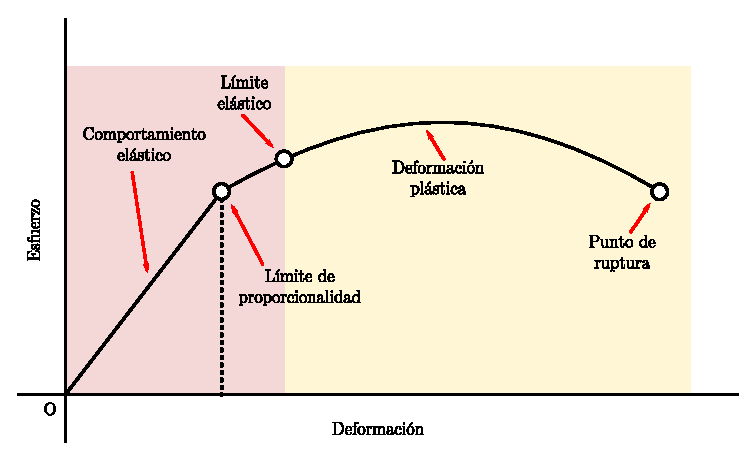
\includegraphics[width=0.80\textwidth]{resources/f1.eps}
\caption{Comportamiento del esfuerzo en función de la deformación.}
\label{figura1}
\source{2013. Sears y Zemansky. Física Universitaria Volumen I. Pagina 358}
\end{figure}

Dentro del limite elástico (donde la ley de \emph{Hooke} es valida), podemos
hallar esa constante propia del material con la siguiente ecuación:

\begin{equation}
    Y = \frac{\sigma}{\epsilon}
\label{young1}
\end{equation}
\vspace{0.25cm}

Donde: $\sigma$ es el esfuerzo, y $\epsilon$ es la deformación unitaria (en este
caso longitudinal para una banda elástica).

Para el calculo de $\sigma$ sabemos que:

\begin{equation}
    \sigma = \frac{F}{A}
\label{sigma}
\end{equation}
\vspace{0.25cm}

Donde: $F$ es la magnitud de la fuerza de tensión realizada, y $A$ el área de la
sección transversal del material.

Mientras que para calcular la deformación unitaria sabemos que:

\begin{equation}
    \epsilon = \frac{L - L_o}{L_o} = \frac{\Delta L}{L_o}
\label{epsilon}
\end{equation}
\vspace{0.25cm}

Donde: $\Delta L$ es la diferencia entre la longitud inicial ($L_o$) del
material y la longitud actual ($L$).

Reuniendo todas las ecuaciones obtenemos \cite{FIS102}:

\begin{equation}
    \frac{F}{A} = Y \frac{\Delta L}{L_o}
\label{young2}
\end{equation}
\vspace{0.25cm}

Para el experimento se tomara los datos del estiramiento de la banda elástica a
diferentes masas de carga, y hasta alcanzar el punto de ruptura; luego se
realizará la gráfica esfuerzo vs. deformación unitaria para una deformación
longitudinal por tensión, de forma que puedan apreciarse las diferentes etapas
de su comportamiento. También se hallará la relación funcional del esfuerzo vs.
deformación unitaria, y finalmente se determinará el módulo de elasticidad del
material.

\section{Método experimental}

Para facilitar la medición, se ha armado el equipo mostrado en la
\textbf{Figura \ref{figura3}}, el cual consta de un \textbf{trípode},
previamente nivelado, y una \textbf{regla de 60 centímetros} (Precisión: 1 [mm])
para facilitar la medición; al trípode se ha sujetado la \textbf{banda elástica}
suspendiendo de esta un contenedor vacío previamente pesado en una
\textbf{balanza} (Precisión: 0.1 [g]).

\begin{figure}
\centering
\includegraphics[width=0.65\textwidth]{resources/f3.eps}
\caption{Montaje del experimento.}
\label{figura3}
\source{Fotografía propia.}
\end{figure}

Una vez montado el soporte, se midió el área de la banda elástica con ayuda de
un \textbf{calibrador} (Precisión: 0.1 [mm]).

Posteriormente se midió la longitud inicial de la banda elástica ya suspendida;
y se procedió a agregar masa al contenedor, a partir de un
\textbf{conjunto de pesos} (en este caso baterías A, AA, y AAA) como los
mostrados en la \textbf{Figura \ref{figura2}}.

\begin{figure}
\centering
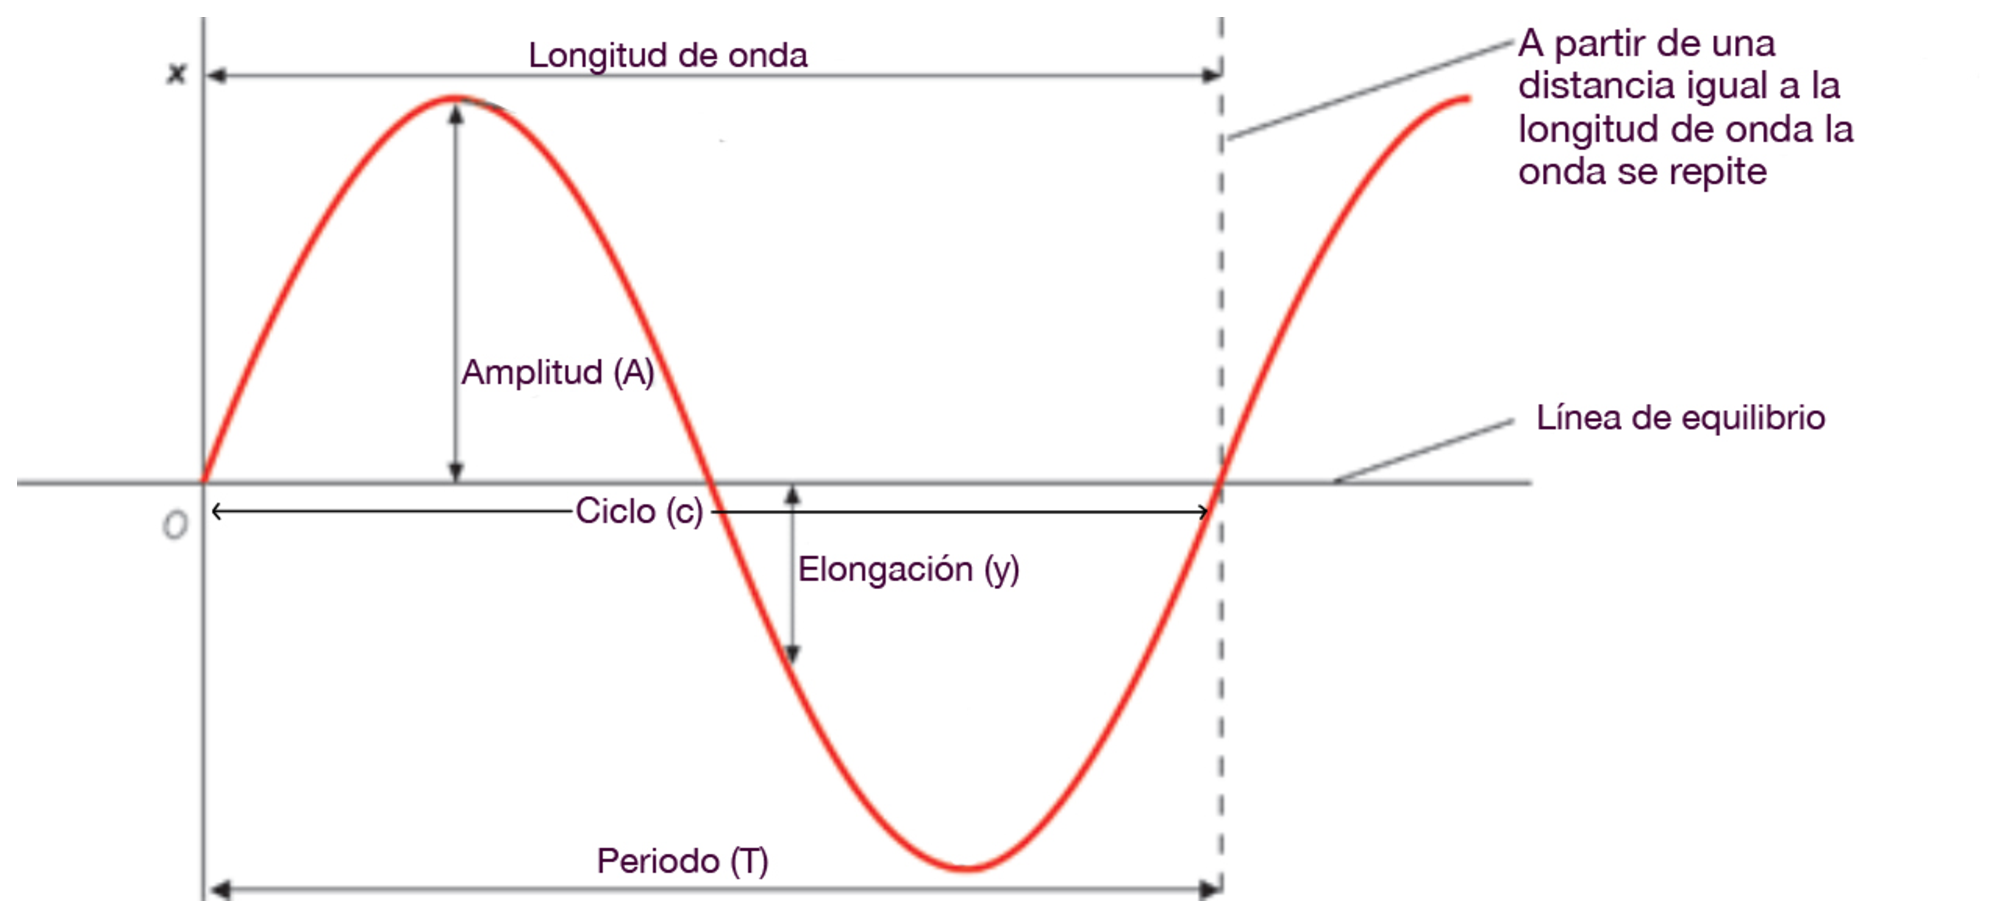
\includegraphics[width=0.65\textwidth]{resources/f2.eps}
\caption{Conjunto de pesos a utilizar.}
\label{figura2}
\source{Fotografía propia.}
\end{figure}

Se registro el incremento de la longitud, hasta alcanzar el punto de ruptura de
la banda elástica.

\vspace{0.35cm}
\textbf{Datos necesarios para el experimento:} \\

Aceleración de la gravedad local:
\begin{equation*}
    g = (9.78 \pm 0.02)[m/s^2]
\end{equation*}

Dimensiones de la banda elástica:
\begin{equation*}
    a_1 = (2.0 \pm 0.1)[mm]
\end{equation*}
\begin{equation*}
    a_2 = (1.6 \pm 0.1)[mm]
\end{equation*}

Longitud inicial de la banda elástica:

\begin{equation*}
    L_o = (0.049 \pm 0.001)[m]
\end{equation*}

\section{Resultados}

En el \textbf{cuadro \ref{cuadro1}}, pueden ver los valores tomados del 
experimento, tanto la masa como la longitud de la deformación resultante:

\begin{table}[!h]
\begin{center}
\begin{tabular}{|c|>{\centering}m{2.5cm}<{\centering}
                  |>{\centering}m{2.5cm}<{\centering}|
                |c|>{\centering}m{2.5cm}<{\centering}
                  |>{\centering}m{2.5cm}<{\centering}|}
\hline
$i$ & $m_i [g]$ & $l_i [cm]$ & $i$ & $m_i [g]$ & $l_i [cm]$ \tabularnewline \hline
\hline
 1 &    0   &  4.1 & 23 &  512.5 & 20.6 \tabularnewline \hline
 2 &   23.4 &  4.6 & 24 &  535.9 & 21.3 \tabularnewline \hline
 3 &   46.9 &  5.5 & 25 &  559.4 & 22.5 \tabularnewline \hline
 4 &   70.0 &  6.4 & 26 &  583.0 & 23.2 \tabularnewline \hline
 5 &   93.1 &  7.5 & 27 &  606.2 & 24.2 \tabularnewline \hline
 6 &  116.4 &  7.9 & 28 &  623.4 & 24.7 \tabularnewline \hline
 7 &  139.6 &  8.9 & 29 &  640.7 & 25.0 \tabularnewline \hline
 8 &  162.9 &  9.8 & 30 &  658.3 & 25.4 \tabularnewline \hline
 9 &  185.7 & 10.8 & 31 &  674.8 & 25.5 \tabularnewline \hline
10 &  207.8 & 11.6 & 32 &  697.1 & 25.8 \tabularnewline \hline
11 &  231.1 & 12.7 & 33 &  733.5 & 26.5 \tabularnewline \hline
12 &  254.4 & 13.5 & 34 &  769.4 & 27.7 \tabularnewline \hline
13 &  277.6 & 14.6 & 35 &  802.3 & 28.0 \tabularnewline \hline
14 &  301.0 & 15.8 & 36 &  837.0 & 29.0 \tabularnewline \hline
15 &  324.3 & 16.2 & 37 &  862.3 & 29.1 \tabularnewline \hline
16 &  347.5 & 17.1 & 38 &  898.2 & 29.5 \tabularnewline \hline
17 &  370.3 & 17.8 & 39 &  932.2 & 29.8 \tabularnewline \hline
18 &  393.6 & 18.1 & 40 &  965.6 & 30.5 \tabularnewline \hline
19 &  420.1 & 19.1 & 41 & 1007.2 & 30.8 \tabularnewline \hline
20 &  443.2 & 19.3 & 42 & 1046.0 & 31.3 \tabularnewline \hline
21 &  466.7 & 19.7 & 43 & 1085.2 & 31.8 \tabularnewline \hline
22 &  489.8 & 20.3 & 44 & 1126.3 & 32.3 \tabularnewline \hline
\end{tabular}
\caption{Mediciones de longitud en función de la masa provista.}
\label{cuadro1}
\source{Elaboración propia.}
\end{center}
\end{table}

A partir de los datos obtenidos se genera la gráfica de la
\textbf{Figura \ref{figura4}} del comportamiento del esfuerzo en función a la
deformación unitaria. Puede verse que el limite de proporcionalidad es próximo
al valor de 3 unidades de deformación unitaria.

\begin{figure}
\centering
\includegraphics[width=0.80\textwidth]{resources/m1.eps}
\caption{Valores del esfuerzo y la deformación unitaria.}
\label{figura4}
\source{Elaboración propia.}
\end{figure}

Por tanto se realizo el ajuste de la curva con las primeras 18 mediciones, por
el método de los mínimos cuadrados, resultando:

\begin{equation*}
    A = (\num{6.8e-10} \pm \num{7.1e-10}) [u]; 100 \%
\end{equation*}
\begin{equation*}
    B = (1.5856 \pm 0.0777) [u]; 4.89 \%
\end{equation*}
\begin{equation*}
    r = 0.9825
\end{equation*}

Sabiendo que el modelo de ajuste es:

\begin{equation*}
    \sigma = a + b \epsilon
\end{equation*}

y despreciando el ínfimo valor de $A$, obtenemos la siguiente relación
funcional:

\begin{equation*}
    \sigma \propto \epsilon
\end{equation*}

Por tanto, el módulo de elasticidad para la banda elástica del experimento es:

\begin{equation*}
    Y = (1.59 \pm 0.08) [N/m^2]; 4.89 \%
\end{equation*}

\section{Discusión}

Si bien los datos obtenidos reflejan claramente las zonas de comportamiento del
material, se debe destacar lo complicado que es agregar masa mientras la banda
elástica se encuentra en la zona plástica, ya que esta comienza a estirarse sin
necesidad de masa adicional, haciendo que las mediciones en esta zona sean muy
imprecisas.

Tuvieron que hacerse tres pruebas antes de la toma de datos, para determinar la
cantidad apropiada de masa a ir agregando de forma que se obtengan suficientes
datos en la zona elástica.

Finalmente al no contar con tantos pesos similares, se tuvieron que realizar
equivalencias de peso para mantener los incrementos de masa constantes, lo que
podría afectar ligeramente las mediciones, dependiendo de la zona en la que este
el material.

Por tal motivo, debe considerarse que el incremento de masa mas apropiado seria
aquel que puede dividirse a grado muy fino, por ejemplo: la arena, o granos de
arroz, de esa forma el control sobre el incremento de masa seria total.

\section{Conclusiones}

Se realizó la gráfica de esfuerzo vs deformación unitaria, en esta puede
apreciarse tanto la zona elástica, como la zona plástica.

Se realizó el ajuste de la curva por el método de mínimos cuadrados y se halló
la relación funcional entre estas dos variables, siendo está constante el
modulo de elasticidad.

\begin{thebibliography}{99}

\bibitem{FIS102} Departamento de Física - UMSS.\\
Laboratorio de Física Básica II.\\
Guía - Cartilla de laboratorio.\\
Gestión I/2020.

\bibitem{Sears y Zemansky} Sears y Zemansky (2013).\\
Física Universitaria. Volumen 1.\\
13va Edición.\\
Capitulo 11.

\end{thebibliography}

\newpage
\section*{Anexo: Cálculos adicionales}

Calculo del área transversal de la banda elástica:
\begin{equation*}
    A = (\num{3.2e-6} \pm \num{2.56e-7})[m^2]
\end{equation*}

Conociendo $L$, $L_o$, $m$, $g$, y $A$, se detallan los valores del esfuerzo
($\sigma$) y la deformación unitaria ($\epsilon$) en el
\textbf{cuadro \ref{cuadro2}}.

\begin{table}[!h]
\begin{center}
\begin{tabular}{|c|>{\centering}m{2.8cm}<{\centering}
                  |>{\centering}m{1.8cm}<{\centering}|
                |c|>{\centering}m{2.8cm}<{\centering}
                  |>{\centering}m{1.8cm}<{\centering}|}
\hline
    $i$ & $\sigma_i [N/m^2] \num{1e6}$ & $\epsilon_i$ & $i$ & $\sigma_i [N/m^2] \num{1e6}$ & $\epsilon_i$ \tabularnewline \hline
\hline
 1 & 0.1247 & 0      & 23 & 1.6910 & 3.3673 \tabularnewline \hline
 2 & 0.1962 & 0.1020 & 24 & 1.7625 & 3.5102 \tabularnewline \hline
 3 & 0.2680 & 0.2857 & 25 & 1.8344 & 3.7551 \tabularnewline \hline
 4 & 0.3386 & 0.4694 & 26 & 1.9065 & 3.8980 \tabularnewline \hline
 5 & 0.4092 & 0.6939 & 27 & 1.9774 & 4.1020 \tabularnewline \hline
 6 & 0.4804 & 0.7755 & 28 & 2.0300 & 4.2041 \tabularnewline \hline
 7 & 0.5513 & 0.9796 & 29 & 2.0828 & 4.2653 \tabularnewline \hline
 8 & 0.6226 & 1.1633 & 30 & 2.1366 & 4.3469 \tabularnewline \hline
 9 & 0.6922 & 1.3673 & 31 & 2.1871 & 4.3673 \tabularnewline \hline
10 & 0.7598 & 1.5306 & 32 & 2.2552 & 4.4286 \tabularnewline \hline
11 & 0.8310 & 1.7551 & 33 & 2.3665 & 4.5714 \tabularnewline \hline
12 & 0.9022 & 1.9184 & 34 & 2.4762 & 4.8163 \tabularnewline \hline
13 & 0.9731 & 2.1429 & 35 & 2.5767 & 4.8776 \tabularnewline \hline
14 & 1.0446 & 2.3878 & 36 & 2.6828 & 5.0816 \tabularnewline \hline
15 & 1.1158 & 2.4694 & 37 & 2.7601 & 5.1020 \tabularnewline \hline
16 & 1.1867 & 2.6531 & 38 & 2.8698 & 5.1837 \tabularnewline \hline
17 & 1.2564 & 2.7959 & 39 & 2.9737 & 5.2449 \tabularnewline \hline
18 & 1.3276 & 2.8571 & 40 & 3.0758 & 5.3878 \tabularnewline \hline
19 & 1.4086 & 3.0612 & 41 & 3.2029 & 5.4490 \tabularnewline \hline
20 & 1.4792 & 3.1020 & 42 & 3.3215 & 5.5510 \tabularnewline \hline
21 & 1.5510 & 3.1837 & 43 & 3.4413 & 5.6531 \tabularnewline \hline
22 & 1.6216 & 3.3061 & 44 & 3.5669 & 5.7551 \tabularnewline \hline
\end{tabular}
\caption{Calculo del esfuerzo y la deformación unitaria.}
\label{cuadro2}
\source{Elaboración propia.}
\end{center}
\end{table}

\end{document}
